\chapter{Theoretical framework}
\label{sec:theoretical_framework}

\section{Graph theory}
This section contains definitions, notation and concepts related to Graph Theory according
to \cite{graph_theory:2010}. \\
Graph theory deals with connection amongst vertices by edges. \\
Graphs are the foundation of many day to day processes and concepts, as they provide a convenient
and intuitive way of representing objects.

\subsection{Simple graphs}
A \textbf{simple graph} \textit{G} consists of a non-empty finite set \textit{V(G)} of elements called \textbf{vertices}
(or \textbf{nodes}), and a finite set \textit{E(G)} of distinct unordered pairs of distinct elements of \textit{V(G)}
called \textbf{edges}. We call \textit{V(G)} the \textbf{vertices set} and \textit{E(G)} the \textbf{edge set} of G.
An edge $\{\textit{v}, \textit{w}\}$ is said to join the vertices v and w, and is usually abbreviated to vw. For example, Figure~\ref{fig:simple_graph} represents the simple graph G whose vertex set \textit{V(G)} is $\{\textit{u}, \textit{v}, \textit{w}, \textit{z}\}$, and whose
edge set \textit{E(G)} consists of the edges \textit{uv}, \textit{uw}, \textit{vw} and \textit{wz}. 

\begin{figure}[H]
    \centering
    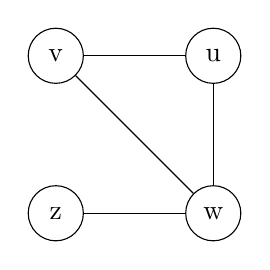
\begin{tikzpicture}
      % Disegno dei nodi
      \node[circle, draw, minimum size=0.7cm] (v) at (0,0) {v};
      \node[circle, draw, minimum size=0.7cm] (u) at (2,0) {u};
      \node[circle, draw, minimum size=0.7cm] (w) at (2,-2) {w};
      \node[circle, draw, minimum size=0.7cm] (z) at (0,-2) {z};
      
      % Disegno degli archi
      \draw (u) -- (v);
      \draw (u) -- (w);
      \draw (v) -- (w);
      \draw (w) -- (z);
    \end{tikzpicture}
    \caption{A simple graph}
    \label{fig:simple_graph}
\end{figure}

\subsection{Adjacency}
We say that two vertices \textit{v} and \textit{w} of a graph \textit{G} are \textbf{adjacent} if there is an edge \textit{vw} joining them, and the vertices \textit{v} and \textit{w} are then \textbf{incident} with such an edge. \\
Similarly, two distinct edges \textit{e} and \textit{f} are \textbf{adjacent} if they have a vertex in common (see Figure \ref{fig:adiacency}).

\begin{figure}[H]
    \centering
    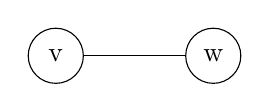
\begin{tikzpicture}
      % Primo grafo
      \node[circle, draw, minimum size=0.7cm] (v) at (0,0) {v};
      \node[circle, draw, minimum size=0.7cm] (w) at (2,0) {w};
      \draw (v) -- (w);
    \end{tikzpicture}
    \quad % Spazio tra i grafi
    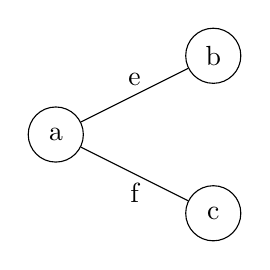
\begin{tikzpicture}
      % Secondo grafo
      \node[circle, draw, minimum size=0.7cm] (a) at (0,0) {a};
      \node[circle, draw, minimum size=0.7cm] (b) at (2,1) {b};
      \node[circle, draw, minimum size=0.7cm] (c) at (2,-1) {c};
      \draw (a) -- node[above] {e} (b);
      \draw (a) -- node[below] {f} (c);
    \end{tikzpicture}
    \caption{Adjacent vertices and adjacent edges}
    \label{fig:adiacency}
\end{figure}

\subsection{Weighted Degree Centrality}
\label{subsec:weighted_degree}
A graph can have 
Weighted degree centrality is a measure used in network analysis to quantify the importance or centrality of a node in a network, taking into account the weights of the edges connected to that node. 
Unlike traditional degree centrality, which only considers the number of connections (edges) a node has, weighted degree centrality considers the strengths or weights associated with those connections.
For a given node, calculate its weighted degree by summing up the weights of all the edges connected to that node. In mathematical terms, it can be expressed as:
\begin{equation}
  WDC(v) = \sum_{i=1}^{N} w_{vi}
\end{equation}
Where \textit{v} is a vertex in the graph and \textit{N} is the number of vertices.

\subsection{Matrix representations}
One approach to representing a graph is through the use of matrices, especially when dealing with large graphs that may not be well-suited for diagram-based representations.\\
Let's consider a graph \textit{G} with \textit{n} vertices and \textit{m} edges. \\
An \textbf{adjacency matrix A} is the $n \times n$ matrix whose \textit{ij}-th entry is the number of edges joining vertex \textit{i} and vertex \textit{j}. \\
If, in addition, the edges are labelled $\{1, 2, \dots, m\}$, its \textbf{incidence matrix M} is the $n \times m$ matrix whose \textit{ij}-th entry is 1 if vertex \textit{i} is incident to edge \textit{j}, and 0 otherwise. \\
An example of this is given in Figure \ref{fig:matrix_representations}.

\begin{figure}[H]
    \centering
    \begin{minipage}{0.5\textwidth}
        \centering
        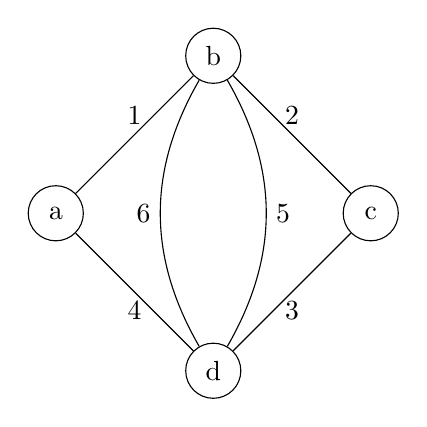
\begin{tikzpicture}
            % Nodi
            \node[circle, draw, minimum size=0.7cm] (a) at (0,0) {a};
            \node[circle, draw, minimum size=0.7cm] (b) at (2,2) {b};
            \node[circle, draw, minimum size=0.7cm] (c) at (4,0) {c};
            \node[circle, draw, minimum size=0.7cm] (d) at (2,-2) {d};
          
            % Archi
            \draw (a) edge node[pos=0.5, below] {4} (d);
            \draw (a) edge node[pos=0.5, above] {1} (b);
            \draw (b) edge[bend left] node[pos=0.5, right] {5} (d);
            \draw (b) edge[bend right] node[pos=0.5, left] {6} (d);
            \draw (b) edge node[pos=0.5, above] {2} (c);
            \draw (c) edge node[pos=0.5, below] {3} (d);
        \end{tikzpicture}
    \end{minipage}%
    \begin{minipage}{0.5\textwidth}
        \[
        A = \begin{bmatrix}
        0 & 1 & 0 & 1 \\
        1 & 0 & 1 & 2 \\
        0 & 1 & 0 & 1 \\
        1 & 2 & 1 & 0
        \end{bmatrix}
        \]
        
        \[
        M = \begin{bmatrix}
        1 & 0 & 0 & 1 & 0 & 0 \\
        1 & 1 & 0 & 0 & 1 & 1 \\
        0 & 1 & 1 & 0 & 0 & 0 \\
        0 & 0 & 1 & 1 & 1 & 1
        \end{bmatrix}
        \]
    \end{minipage}
    \caption{Graph \textit{G} with its adjacency \textit{A} and incidence \textit{M} matrices}
    \label{fig:matrix_representations}
\end{figure}


\subsection{Bipartite graphs}
If the vertex set of a graph \textit{G} can be split into two disjoint sets \textit{A} and \textit{B} so that each
edge of \textit{G} joins a vertex of \textit{A} and a vertex of \textit{b}, then \textit{G} is a \textbf{bipartite graph}. \\
Alternatively, a bipartite graph is one whose vertices can be coloured red and blue in such a way that each edge joins a red vertex (in \textit{A}) and a blue vertex (in \textit{B}). \\

\begin{figure}[H]
    \centering
    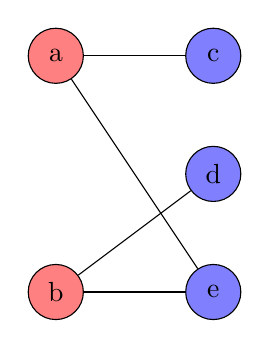
\begin{tikzpicture}[every node/.style={circle, draw, minimum size=0.7cm}]
        % Livello superiore
        \node (A) at (3,0) [fill=red!50] {a};
        \node (B) at (3,-3) [fill=red!50] {b};
        
        % Livello inferiore
        \node (C) at (5,0) [fill=blue!50] {c};
        \node (D) at (5,-1.5) [fill=blue!50] {d};
        \node (E) at (5,-3) [fill=blue!50] {e};
        
        % Collegamenti
        \draw (A) -- (C);
        \draw (A) -- (E);
        \draw (B) -- (D);
        \draw (B) -- (E);
    \end{tikzpicture}
    \caption{A simple bipartite graph}
    \label{fig:bipartite}
\end{figure}



\subsection{Bipartite graphs with matching}
A \textbf{bipartite graph with matching} is a bipartite graph in which there is a set of edges selected in such a way that no node is shared among the edges of the matching.
In other words, each node is involved in at most one edge of the matching. \\
This means that if the number of vertices in \textit{A} and \textit{B} is different, at least one vertex will have no connection to another vertex (see Figure \ref{fig:match_1}). \\
If there is the same number of vertices in both \textit{A} and \textit{B}, every vertex is connected to another vertex (see Figure \ref{fig:match_2}). \\

\begin{figure}[H]
  \centering
  \begin{subfigure}{0.48\linewidth}
    \centering
    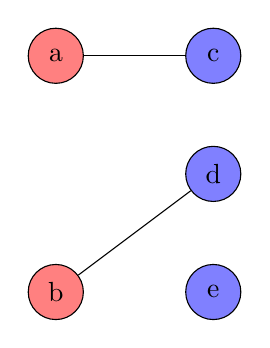
\begin{tikzpicture}[every node/.style={circle, draw, minimum size=0.7cm}]
      % Livello superiore
      \node (A) at (3,0) [fill=red!50] {a};
      \node (B) at (3,-3) [fill=red!50] {b};

      % Livello inferiore
      \node (C) at (5,0) [fill=blue!50] {c};
      \node (D) at (5,-1.5) [fill=blue!50] {d};
      \node (E) at (5,-3) [fill=blue!50] {e};

      % Collegamenti
      \draw (A) -- (C);
      \draw (B) -- (D);
    \end{tikzpicture}
    \caption{}
    \label{fig:match_1}
  \end{subfigure}
  \hspace{0.02\linewidth}
  \begin{subfigure}{0.48\linewidth}
    \centering
    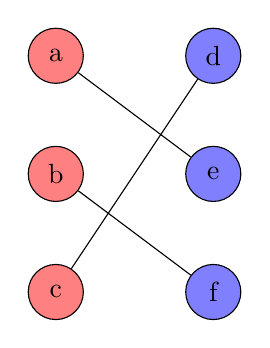
\begin{tikzpicture}[every node/.style={circle, draw, minimum size=0.7cm}]
      % Livello superiore
      \node (A) at (3,0) [fill=red!50] {a};
      \node (B) at (3,-1.5) [fill=red!50] {b};
      \node (C) at (3,-3) [fill=red!50] {c};

      % Livello inferiore
      \node (D) at (5,0) [fill=blue!50] {d};
      \node (E) at (5,-1.5) [fill=blue!50] {e};
      \node (F) at (5,-3) [fill=blue!50] {f};

      % Collegamenti
      \draw (A) -- (E);
      \draw (B) -- (F);
      \draw (C) -- (D);
    \end{tikzpicture}
    \caption{}
    \label{fig:match_2}
  \end{subfigure}
  \caption{Bipartite graph}
\end{figure}

\subsection{Maximum Weight Perfect Matching}
\label{sec:MaxWPM}
The Maximum Perfect Weight Matching is an optimization problem concerning graphs.
The graphs in question are bipartite, meaning the vertices can be divided into two distinct sets in such a way that all edges of the graph connect vertices from different sets, with no edges connecting vertices within the same set.
Additionally, these graphs are undirected, meaning the relationship between two nodes is bidirectional, in other words, the edge connecting node A to node B automatically implies the existence of the edge connecting node B to node A. \\
In the MaxWPM problem, the vertices represent elements to be paired, and the edges represent possible connections between these elements. 
Each edge is associated with a weight that represents the value or importance of the pairing between the connected vertices.\\
The goal is to find a perfect matching, which is a set of edges in which every node is connected to exactly one other node, with no overlaps or isolated nodes, while maximizing the total weight of the edges in the matching.
The total weight is the sum of the weights of the edges included in the matching.
The weights of the edges are collected in a matrix called a \textit{utility matrix}.\\
The utility matrix will be a square matrix because the number of nodes in the two distinct sets is the same.
The rows could represent the nodes in the first set, while the columns could represent the nodes in the second set, or vice versa.
The element (\textit{i}, \textit{j}) of the matrix represents the weight of the edge connecting vertex \textit{i} to vertex \textit{j}. 


A MaxWPM problem using an utility matrix can be transformed into a \textbf{Minimum Weight Perfect Matching} problem.
This can be achieved by introducing an auxiliary matrix, referred to as the \textit{cost matrix}.
The cost matrix is essentially a duplicate of the utility matrix, but with all its elements negated.

\section{Brute Force Algorithm}
The BF can be a possible approach to solve the MaxWPM problem for bipartite graphs.
However, it's important to note that the BF has exponential time complexity, specifically, its time complexity grows exponentially with the number of vertices in the graph.
This is because the BF examines all possible combinations of matchings within the bipartite graph to find the one with the maximum weight.\\
If the graph has \textit{n} vertices in both the first and second partitions, there are \textit{n}!\ possible matchings.
Each matching requires \textit{O}(\textit{n}) time to be computed because you need to check that it is a perfect matching and calculate its total weight.
Therefore, the overall complexity of the algorithm is on the order of \textit{O}(\textit{n}!$\cdot$\textit{n}). \\
Since the complexity grows rapidly as \textit{n} increases, it quickly becomes impractical for large-sized graphs. \\

The operation of the BF for MinWPM problems can be summerized in these 3 steps:

\begin{enumerate}
    \item {Compute the cost matrix for the considered bipartite graph with \textit{n} vertices in each partition.}
    \item {Compute the total cost of all the \textit{n}!\ permutations.}
    \item {Choose the assignment with the lowest total cost.}
\end{enumerate}


\subsection{Hungarian Matching Algorithm}

The HM, also called the Kuhn-Munkres algorithm, is a \textit{O}($\textit{n}^3$) algorithm that can be used to find MaxWPM in bipartite graphs with \textit{n} vertices for each partition, which is sometimes called the assignment problem.
As previously demonstrated in the Brute Force algorithm, maximum-weight perfect matching problems using the utility matrix can be converted into MinWPM problems using the cost matrix. 
We will describe the application of the HM to address Minimum Weight Perfect Matching problems. \\

The operation of the HM for MinWPM problems can be summerized in these 6 steps:
\begin{enumerate}
    \item {Compute the cost matrix for the considered bipartite graph with \textit{n} vertices in each partition.}
    \item {Subtract the smallest entry in each row from all the other entries in the row. This will make the smallest entry in the row now equal to 0.}
    \item {Subtract the smallest entry in each column from all the other entries in the column. This will make the smallest entry in the column now equal to 0.}
    \item {Draw lines through the row and columns that have the 0 entries such that the fewest lines possible are drawn.}
    \item {If there are n lines drawn, an optimal assignment of zeros is possible and the algorithm is finished. If the number of lines is less than n, then the optimal number of zeroes is not yet reached. Go to the next step.}
    \item {Find the smallest entry not covered by any line. Subtract this entry from each row that isn’t crossed out, and then add it to each column that is crossed out. Then, go back to Step 3.}
\end{enumerate}



\section{Game theory}
Game theory is a type of decision theory in which one’s choice of action is determined after taking
into account all possible alternatives available to an opponent playing the same game, rather than just
by the possibilities of several outcome results. \\
Game theory does not insist on how a game should be played but tells the procedure and principles by which action should be selected.
Thus it is a decision theory useful in competitive situations. \\
Game is defined as an activity between two or more persons according to a set of rules at the end of
which each person receives some benefit or suffers loss. The set of rules defines the game.
Going through the set of rules once by the participants defines a play.
\\

The following sections contains notations and properties accordind to \cite{game_theory:2020}.

\subsection{Properties of a Game}
\begin{enumerate}
    \item {There are finite numbers of competitors called \textit{players}.}
    \item {Each player has a finite number of possible courses of action called \textit{strategies}.}
    \item {All the strategies and their effects are known to the players but player does not know which
    strategy is to be chosen.}
    \item {A game is played when each player chooses one of his strategies. The strategies are assumed
    to be made simultaneously with an outcome such that no player knows his opponents strategy
    until he decides his own strategy.}
    \item {The game is a combination of the strategies and in certain units which determines the gain or
    loss.}
    \item {The figures shown as the outcomes of strategies in a matrix form are called \textit{pay-off matrix}.}
    \item {The player playing the game always tries to choose the best course of action which results in
    optimal pay off called \textit{optimal strategy}.}
    \item {The expected pay off when all the players of the game follow their optimal strategies is
    known as \textit{value of the game}. The main objective of a problem of a game is to find the value
    of the game.}
    \item {The game is said to be \textit{fair} game if the value of the game is zero otherwise it's known as \textit{unfair}.}
    \item {A \textit{coalition} is a subset of the players \textit{n}, whereas a \textit{grand coalition} is the
        set \textit{n} of all players. The purpose of a coalition is to coordinate strategies and divide the
        total payoff among all the players.}
\end{enumerate}


\subsection{Cooperative Games}
A cooperative game is a situation in which players interact together to achieve a common goal.
In the context of a cooperative game, players aim to maximize the overall outcome by collaborating, communicating, and coordinating their actions.
The primary objective is to achieve a result in which all players benefit, working together to overcome challenges or issues.


\subsection{Non-cooperative Games}
A non-cooperative game is a situation in which players act independently and without direct communication or coordination with other players.
In a non-cooperative game, each player seeks to maximize their individual gain without necessarily considering the effect of their actions on other players.
The main goal is to achieve the best personal outcome, even at the expense of other participants, without considering direct collaboration.


\section{Machine Learning Theory}
\label{subsec:ML}

ML deals with the ability of a system to improve its performance through experience, without being explicitly programmed.
It also serves as the foundation for numerous everyday applications and concepts, 
as it provides a powerful and efficient way to address complex challenges, make data-driven decisions, 
and develop intelligent systems that can learn and adapt autonomously.\\

Diving deeper into this concept, one critical aspect is the role of hyperparameters. 
Hyperparameters are settings or configurations that guide the learning process of ML algorithms. 
They act as the levers that fine-tune the behavior of these algorithms, influencing their performance, accuracy, and generalization capabilities.\\
Hyperparameters encompass a wide range of choices, such as the learning rate in gradient descent, the depth of a decision tree, the number of hidden layers in a neural network, or the number of clusters in a k-means clustering algorithm. 
Selecting the right hyperparameters can be a challenging and often iterative task, as they significantly impact the model's ability to capture underlying patterns in data.\\
The process of hyperparameter tuning involves experimenting with different combinations of values, assessing the model's performance using techniques like cross-validation, and iteratively adjusting the hyperparameters to optimize the model's accuracy and generalization. 
This fine-tuning is crucial to ensure that the ML model not only fits the training data well but also performs effectively on unseen data.
Moreover, the choice of hyperparameters is problem-dependent, and there's no one-size-fits-all solution. 
It requires a deep understanding of the algorithm, the dataset, and the specific problem at hand.saisi

\subsection{Classifier}
\label{subsec:classifier}

A mathematical \textbf{Classifier} is a model that takes an input dataset and assigns each data point to a class or category. 
The mathematical formulation of a classifier can vary depending on the algorithm used. 
Suppose we have a training dataset represented as pairs (\textit{$\overline{x}$}, \textit{y}), where \textit{$\overline{x}$} is a vector of data features, and \textit{y} is the associated class label.
The \textit{y} is a categorical (can take a fixed, number of possible values) variable that categorizes between two or more classes ('dog', 'cat', 'bird'), while in a regression problem it is a continuous variable.
Our goal is to find a function \textit{f}(\textit{$\overline{x}$}) that maps the feature vectors \textit{$\overline{x}$} to class labels \textit{y}. \\

A \textbf{Binary Classification Problem} is a specific type of classification problem where the goal is to categorize input data into one of two distinct classes or categories. 
These two classes are typically referred to as the positive class and the negative class, and the task is to assign each data point to one of these two classes based on its features or attributes.
\begin{figure}[H]
  \centering
  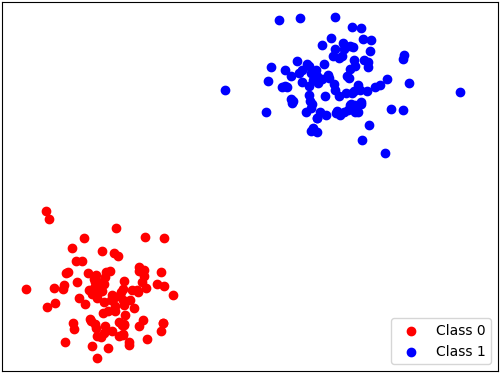
\includegraphics[width=0.6\linewidth]{graphics/BinaryClassification.png}
  \caption{Binary Classification example}
  \label{fig:bin_classification}
\end{figure}

\subsection{K-Nearest Neighbors}
\label{subsec:KNN}

The \textbf{KNN} algorithm is a supervised ML algorithm used for classification and regression tasks.
It is a simple and intuitive algorithm that makes predictions based on the similarity between a data point and its k-nearest neighbors in a training dataset.
The \textit{k} in \textit{k}-nearest neighbors refers to the number of items that the algorithm uses to make its prediction whether its a classification problem or a regression problem.
In Figure \ref{fig:knn} we can see a test sample represented by a green dot and we want to classify 
it either as a blue square or a red triangle based on a KNN algorithm, the decision depends on the value of \textit{k}, which determines how many nearest neighbors we consider.\\
When \textit{k} = 3 (solid line circle), the green dot is assigned to the category that has the majority among its three nearest neighbors. 
In this case, if there are 2 red triangles and only 1 blue square inside the inner circle, the green dot is classified as a red triangle. \\
When \textit{k} = 5 (dashed line circle), the green dot is assigned to the category with the majority among its five nearest neighbors. 
If there are 3 blue squares and 2 red triangles inside the outer circle, the green dot is classified as a blue square.
\begin{figure}[H]
    \centering
    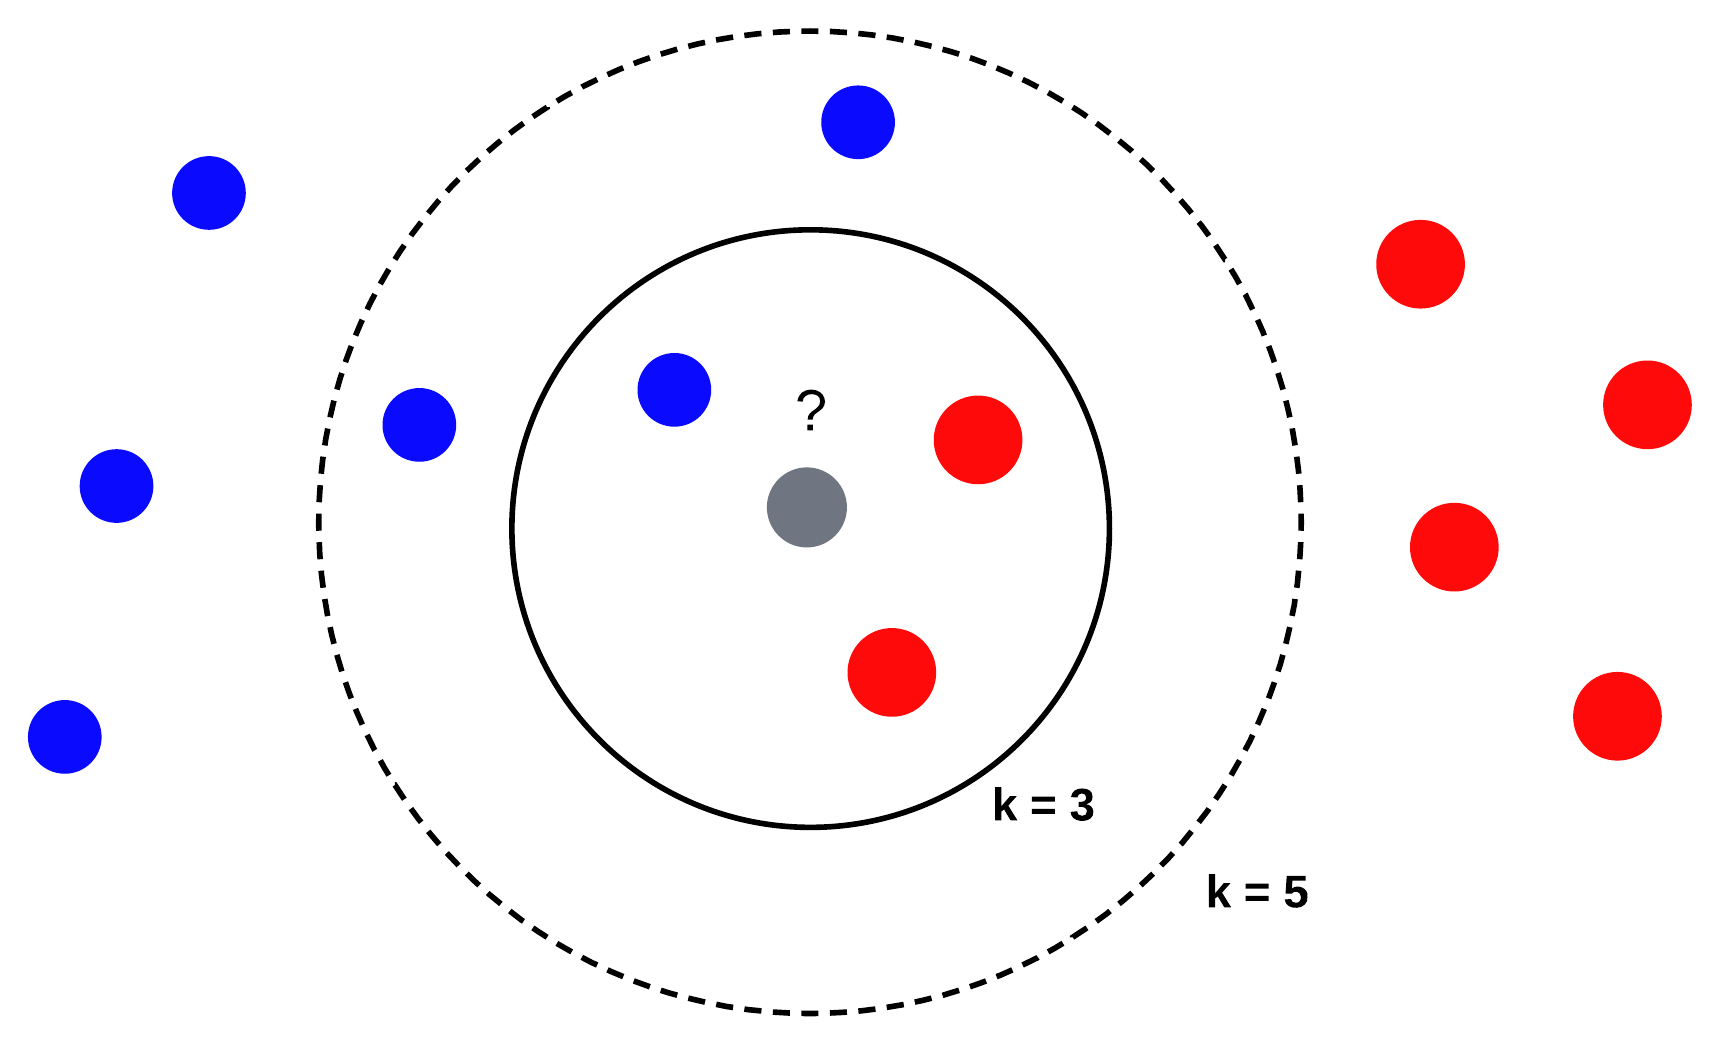
\includegraphics[width=0.55\linewidth]{graphics/KNeighbours.png}
    \caption{KNN algorithm with \textit{k} = 3 and \textit{k} = 5}
    \label{fig:knn}
\end{figure}

The choice of distance metric is a critical aspect of the KNN algorithm, and while it's not typically considered a hyperparameter, it significantly influences the model's performance and outcomes. 
The selection of a specific distance metric can have a substantial impact, especially when dealing with datasets of varying sizes and dimensions. \\
If we consider for example two data points \textit{p}, \textit{q} in \textit{n}-dimensional space, there are various distance metrics that can be used to find the neighbors.\\
Among the different  most common is the Euclidean distance: 
\begin{equation}
    Euclidean(p,q) = \sqrt{\sum_{i=1}^{n} (p_i - q_i)^2}
    \label{formula:distance}
\end{equation}

\subsection{Borderline Synthetic Minority Over-sampling Technique}
\label{subsec:borderline}

\textbf{Oversampling} is a technique used in the field of imbalanced ML to address the problem of class imbalance. 
Class imbalance occurs when one class in a classification problem has significantly fewer instances than another class. 
This imbalance can lead to biased models that perform poorly on the minority class (the class with fewer instances) because the model tends to be biased towards the majority class.\\
The concept of oversampling involves increasing the number of instances in the minority class by generating synthetic or duplicate samples. 
The goal is to balance the class distribution, making the minority class more comparable in size to the majority class. 
A synthetic sample can be generated duplicating randomly another sample of the minority class or considering its underlying data distribution (ADASYN \cite{adasyn:2008}).
This could result in a performance improvement of ML models by providing them with more information about the minority class.\\
The SMOTE generates synthetic samples by interpolating between neighboring minority class instances using an underlying KNN model.\\

The \textbf{B-SMOTE} \cite{Han2005BorderlineSMOTEAN:2005}, is a vairant of the SMOTE that focuses on generating synthetic samples only for the boundary instances, which are the minority class instances close to the majority class. 
This approach aims to concentrate on the regions of the dataset that are near the decision boundary between classes. \\
The model internally fits two instances of KNN with different \textit{k} parameters (\textit{k-neighbors}, \textit{m-neighbors}): one instance to defines the neighborhood of samples to generate the synthetic samples.
The other instead is used to determine if a minority sample is in \textit{danger}. A \textit{sample in danger} is one near to the boundary between two or more classes.

In the illustrated scenario depicted in Figure \ref{fig:bordSMOTEnotApplied}, the task involves categorizing two distinct categories of network traffic: 
one being malicious (depicted in red), the other representing legitimate traffic (shown in blue), and the decision boundaries are the same color meshes.
The distribution of malicious traffic is more sparse and rare compared to legitimate traffic, this means that the classifier has been trained on an imbalanced dataset. 
The primary objective of the classification is to maximize the detection of malicious traffic, even if it entails misclassifying some instances of legitimate traffic. 
BSMOTE is a possible solution for this scenario, where the two classes are significantly imbalanced, and the weight of legitimate traffic in the classification process could be overwhelming.

The application of the BSMOTE algorithm facilitates class rebalancing by generating synthetic data points in the boundary regions between the classes concentrated in proximity of the decision boundary.
In Figure \ref{fig:bordSMOTEApplied}, the depicted image showcases the ultimate outcome achieved following the retraining of the classifier. 
The retraining process maintained the same parameters but employed a dataset that has been more uniformly balanced.
The synthetic samples generated by BSMOTE are represented as light-red dots.
\begin{figure}[H]
  \centering
  \begin{subfigure}{0.45\linewidth}
    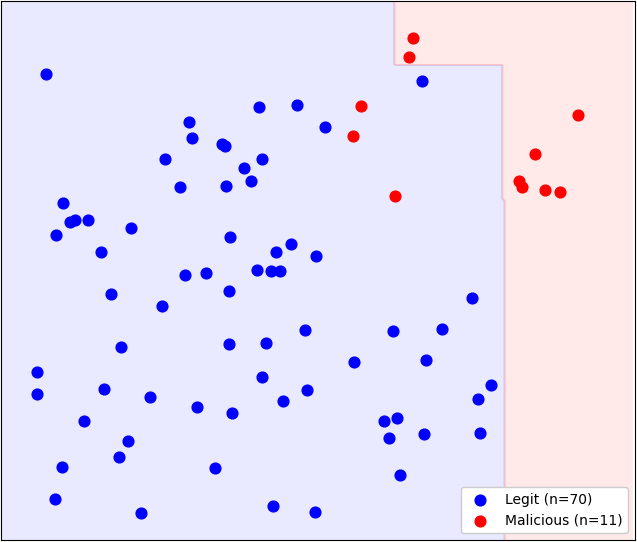
\includegraphics[width=\linewidth]{graphics/BordSMOTE_no.png}
    \caption{}
    \label{fig:bordSMOTEnotApplied}
  \end{subfigure}
  \hspace{0.01\linewidth}
  \begin{subfigure}{0.45\linewidth}
    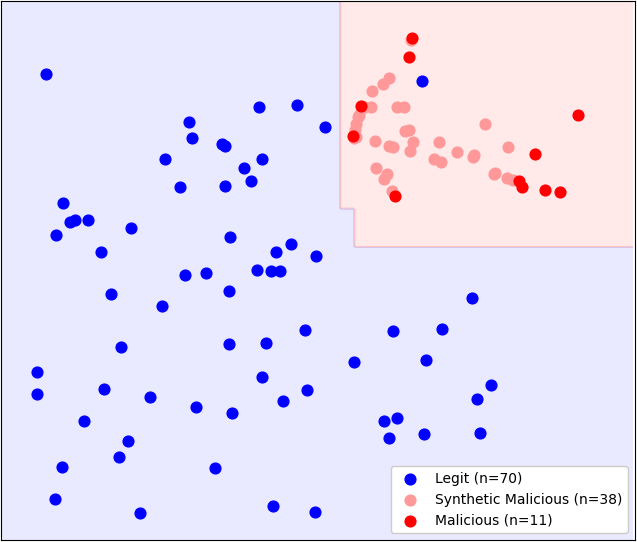
\includegraphics[width=\linewidth]{graphics/BordSMOTE_yes.png}
    \caption{}
    \label{fig:bordSMOTEApplied}
  \end{subfigure}
  \caption{Visual representation of BSMOTE algorithm applied on a dataset}
\end{figure}

However The BSMOTE algorithm, like any other method, has its limitations and drawbacks:
\begin{itemize}
  \item \textbf{Risk of Overfitting:} In the provided example, the malicious data was generated using a normal distribution, while the legitimate data was generated using a uniform distribution.
  This means that the second classification fits better the underlying distribution without any a-priori assumption.
  But in some cases depending on the choice of borderline examples, 
  BSMOTE may introduce a bias towards certain patterns or classes in the synthetic samples, which can affect the model's generalization.
  It can potentially lead to overfitting, especially when it generates a large number of synthetic samples in the borderline region. 
  This may cause the model to perform exceptionally well on the training data but poorly on unseen data.
  \item \textbf{Computationally intensive:} It can require high hardware resources, especially in high-dimensional spaces, as it involves calculating distances between data points. 
  This can lead to longer training times, making it less suitable for large datasets.
  \item \textbf{Designed for Clearly Separable Datasets:} It is designed for datasets with clear class boundaries and is most effective when the borderline instances are well-defined. 
  In cases where class separation is not distinct, it may not provide substantial benefits.
\end{itemize}
So in general, even if it aims to improve the classification of the minority class, there is no guarantee that it will always lead to better results.

\subsection{Random Forest Classifier}
\label{subsec:RF}

A \textbf{Decision Tree} (DT) is a non-parametric supervised learning algorithm, which is utilized for both classification and regression tasks. 
It has a hierarchical, tree structure, which consists of a internal nodes, leaf nodes and branches.
From the root node, splitting criterias are applied on the samples creating branches and child nodes that lead to leaf nodes which represent the final classification of the tree.
The most common impurity measure used to quantify the impurity of a dataset is the Gini criterion:
For a set of items with \textit{J} classes and relative frequencies $p_{i}$, $i \in {1,2,...,J}$ 
the probability of choosing an item with label $i$ is $p_{i}$, and the probability of miscategorizing that item is:
\begin{equation} 
  \sum_{k \ne i} p_{k} = 1 - p_{i} 
\end{equation}
The Gini impurity is computed by summing pairwise products of these probabilities for each class label:
\begin{equation}
  Gini(p) = 1 - \sum_{i=1}^{J} (p_i^2)
\end{equation}

In the example shown in Table \ref{tab:tableDecisionTreeDataset}, the objective is to determine whether to grant a loan based on two pieces of information: 
the applicant's monthly income and the requested loan amount. The second figure illustrates the DT that has been trained on this dataset.
The underlying principle of the DT is that at every non-terminal node, if there exist samples that need further separation, the following algorithm is applied: 
\begin{enumerate}
  \item It starts by calculating the impurity of the current node before making any splits. This initial impurity serves as a baseline for evaluating feature splits.
  \item For each feature in the dataset, calculate a measure of impurity or information gain for potential splits. This typically involves examining the feature values and considering different threshold values.
  \item Calculates the reduction in impurity (or information gain) achieved by the potential split. This is done by comparing the impurity of the current node with the impurity of the child nodes created by the split.
  \item Choose the feature that results in the highest information gain. This feature becomes the one on which to apply the threshold for the split.
  \item It applies the threshold that separates the data into two or more subsets.
  \item Continue the process recursively for each child node created by the split. This means repeating steps 1 to 5 for each child node until a stopping criterion is met (e.g., a maximum tree depth is reached).
\end{enumerate}
The goal is to create child nodes that are as homogeneous as possible with respect to the target variable, thereby improving the predictive accuracy of the tree.
\begin{table}[H]
  \centering
  \begin{tabular}{|>{\centering\arraybackslash}p{3.2cm}|>{\centering\arraybackslash}p{3.2cm}|>{\centering\arraybackslash}p{3.2cm}|}
  \hline
  \textbf{Income} & \textbf{Loan\_Amount} & \textbf{Loan\_Approved} \\
  \hline
  2000 & 300000 & Not Approved \\
  3000 & 300000 & Approved \\
  4000 & 400000 & Not Approved \\
  5000 & 400000 & Not Approved \\
  10000 & 400000 & Approved \\
  15000 & 400000 & Approved \\
  \hline
  \end{tabular}
  \caption{Dataset of the DT}
  \label{tab:tableDecisionTreeDataset}
\end{table}
\begin{figure}[H]
  \centering
  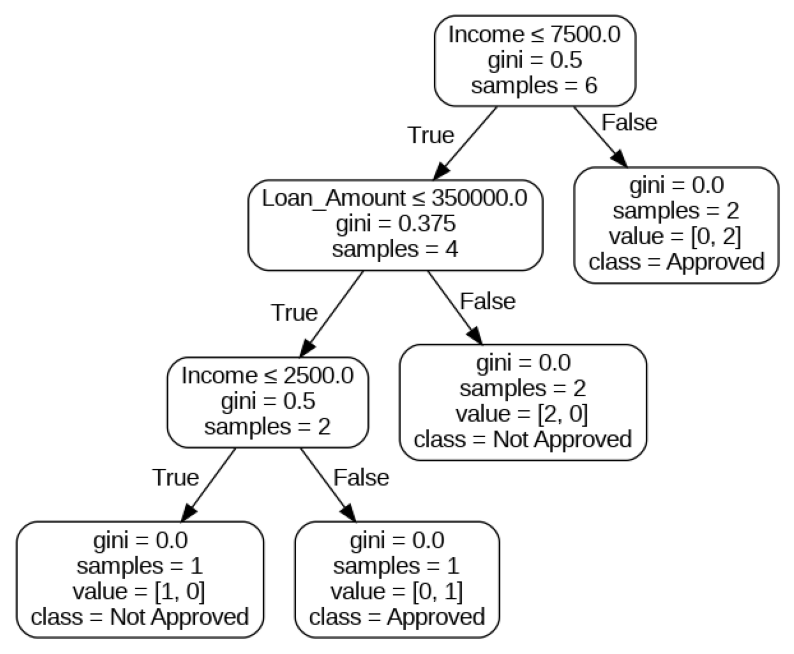
\includegraphics[width=0.6\linewidth]{graphics/DecTree.png}
  \label{fig:knn5}
  \caption{DT applied on the dataset of Table \ref{tab:tableDecisionTreeDataset}}
\end{figure}
In the example provided the term “samples" represent the total number of training samples used to create the specific tree node. 
In other words, it is the number of data examples that were considered in that node during the tree construction process.

Note that due to the absence of constraints on hyperparameters like tree depth or the minimum number of features required to split nodes, 
it becomes evident that each sample in the dataset follows a distinct path within this tree. 
The term “value" represents the distribution of classes or labels of the samples within a node. 
It is a vector that indicates how many training samples in that node belong to each class or category. 
For instance, if we see “value = [0, 2]," it means that there are 0 samples belonging to class “Not Approved" and 2 samples belonging to class “Approved" in that node.
This example is simply used for showing the behaviour of a DT\\

\textbf{Random Forest} is an ensemble learning method that builds multiple DTs during training and combines their predictions to make more accurate and robust classifications or regressions.
A RF is typically constructed in this way:
\begin{enumerate}
  \item \textbf{Bootstrapped Data:} A random subset of the training data (with replacement) is used to train each DT. This results in each tree being trained on a slightly different dataset.
  \item \textbf{Random Feature Selection:} At each node of each DT, only a random subset of the available features is considered for splitting. This helps introduce diversity among the trees and reduces the risk of overfitting.
  \item \textbf{Independent Training:} Each DT is trained independently. There is no communication or shared information between the trees during training.
  \item \textbf{Voting or Averaging:} For classification tasks, the RF combines the individual tree predictions by applying a Majority Voting (each tree "votes" for a class and the final prediction reflects the class that receives the most votes overall)
\end{enumerate}
The key idea behind the RF method is that by aggregating the predictions of multiple DTs, the ensemble can reduce overfitting, improve generalization, and provide more robust and accurate results.
For example the Figure \ref{fig:rf} is shown a RF classifier made of 3 DTs has been created applying the bootstrap method on the dataset and correctly classifies the first sample of the dataset in Table \ref{tab:tableDecisionTreeDataset}.

\begin{figure}[H]
  \centering
  \begin{subfigure}{0.45\linewidth}
    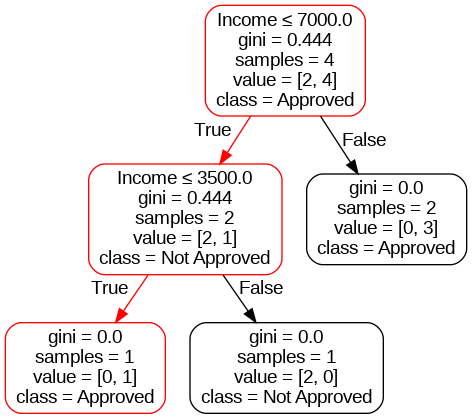
\includegraphics[width=\linewidth]{graphics/loan_RF_1.png}
    \caption{}
    \label{fig:rfTree0}
  \end{subfigure}
  \hspace{0.06\linewidth}
  \begin{subfigure}{0.45\linewidth}
    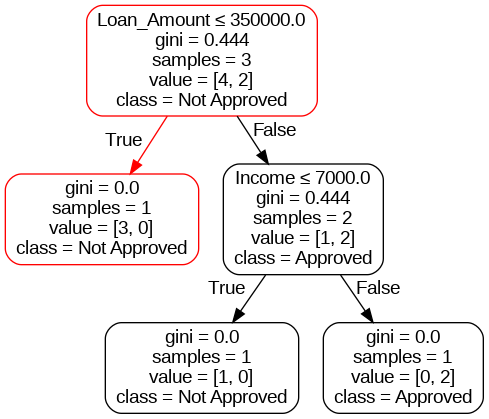
\includegraphics[width=\linewidth]{graphics/loan_RF_2.png}
    \caption{}
    \label{fig:rfTree1}
  \end{subfigure}
  \begin{subfigure}{0.39\linewidth}
    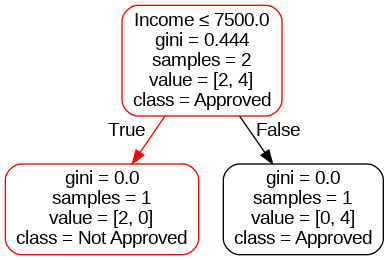
\includegraphics[width=\linewidth]{graphics/loan_RF_0.png}
    \caption{}
    \label{fig:rfTree2}
  \end{subfigure}
  \caption{Path taken by the first sample through the three DTs of a RF classifier}
  \label{fig:rf}
\end{figure}


\subsection{Cross Validation}
\label{subsec:cross_validation}

\textbf{Cross Validation} is a technique used to estimate the effectiveness of a ML model based on a data sample.
It involves dividing the dataset into multiple training and testing subsets called \textit{folds} and then training and evaluating the model on each fold.
The process of training and testing is typically repeated multiple times and the results from each iteration are often averaged to provide an overall estimate of the model's performance.
The most common approach in basic cross-validation is to use a 80-20 or 70-30 split between the training and test sets.\\
When we partition our dataset into folds for techniques like cross-validation, it's crucial to ensure that each fold accurately represents the diversity of the entire dataset. 
This entails maintaining the same proportion of different classes or categories within each fold.\\ 
While random splitting is often sufficient, there are instances, particularly in intricate datasets, where we must deliberately enforce the correct distribution of classes within each fold to maintain data integrity.
\\

\textbf{Leave-One-Out Cross-Validation} (LOOCV) is a specific type of cross-validation where the number of folds $k$ is set equal to the number of samples in the dataset $n$. 
In this approach, the model undergoes training k times, with k being precisely the total number of samples $n$.
During each of the \textit{k} iterations, a distinct sample is singled out as the test set, while all the remaining samples are utilized for model training. 
This procedure ensures that every single sample gets its turn as the test set, comprehensively assessing the model's performance across the entire dataset.
In Figure \ref{fig:LOOCV} is shown how it works, note that training is performed on the same model at each iteration and 

\begin{figure}[H]
  \centering  
    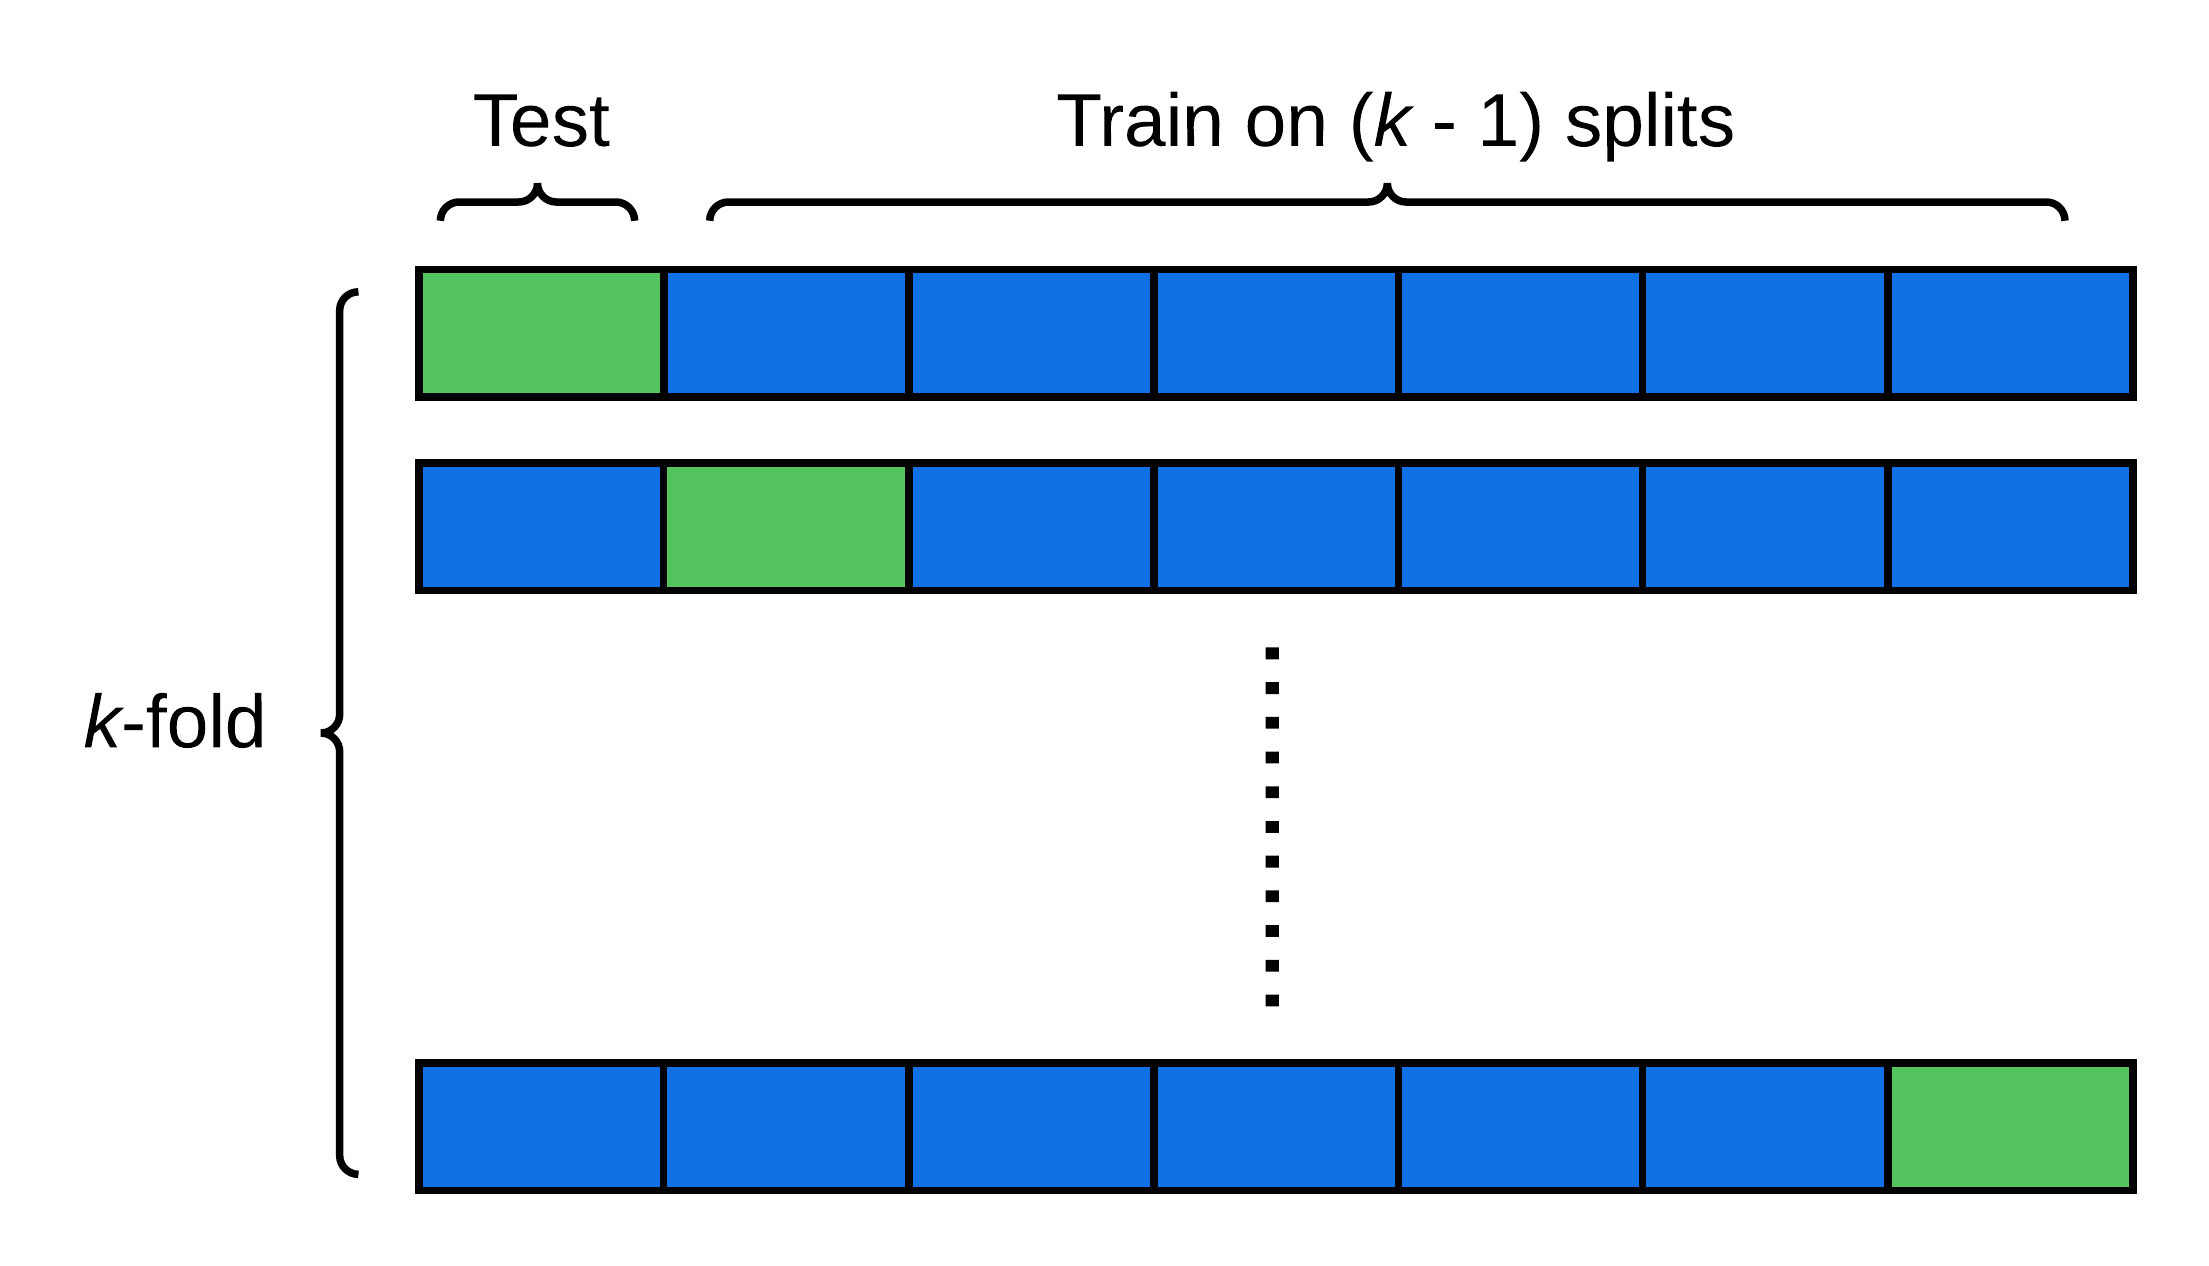
\includegraphics[width=0.8\linewidth]{graphics/LOOCV.png}
    \caption{LOOCV algorithm example on \textit{k} folds}
    \label{fig:LOOCV}
\end{figure}
However, LOOCV has some downsides:
\begin{itemize}
  \item \textbf{Computational Cost:} It can be computationally expensive, especially on large datasets, as it requires a significant number of separate model trainings. 
  Training the model repeatedly for each sample can be time-consuming and resource-intensive.
  \item \textbf{Variance:} In some cases, LOOCV may have high variance because it relies on the performance of a single sample as the test set in each iteration. 
  This can lead to variability in the estimated performance.
\end{itemize}  
    
\subsection{Evaluation Metrics}
\label{subsec:evaluation_metrics}

Evaluation metrics in ML are fundamental tools for measuring the effectiveness and accuracy of predictive models.
These metrics provide a clear overview of the model's performance and assist in making informed decisions during the development and optimization process. \\

The \textbf{confusion matrix} is an essential tool used in the evaluation of classification models in ML.
It provides a detailed overview of a model's performance by comparing the model's predictions with the actual class labels of the test data. \\
The confusion matrix consists of four main elements:

\begin{enumerate}

\item{\textbf{True Positives (TP)}: The model correctly predicted a positive class. 
For example, if we are trying to identify spam emails, and the model correctly classified an email as spam, it is a True Positive.}
\item{\textbf{True Negatives (TN)}: The model correctly predicted a negative class.}
\item{\textbf{False Positives (FP)}: The model incorrectly predicted a positive class when it was actually negative. This is also referred to as \textit{Type I error}.} 
\item{\textbf{False Negatives (FN)}: The model incorrectly predicted a negative class when it was actually positive. This is also referred to as \textit{Type II error}.}
\end{enumerate}

\begin{figure}[H]
  \centering
  \renewcommand{\arraystretch}{2} % Aumenta lo spazio tra le righe del doppio
  \begin{tabular}{|>{\rule[-0.5cm]{0pt}{1.5cm}}c|c|c|}
  \hline
  \backslashbox{Real}{Pred} & Negative &  Positive\\
  \hline
  Negative & TN & FP \\
  \hline
  Positive & FN & TP \\
  \hline
  \end{tabular}
  \caption{Example of confusion matrix}
  \label{tab:conf_matrix}
\end{figure}

The confusion matrix is an important resource for calculating various evaluation metrics such as:


\begin{itemize}
  \item{

  \textbf{Accuracy} is a measure of the overall percentage of correct predictions made by a classification model.

  \begin{equation}
    \textit{Accuracy} = \frac{\text{TP + TN}}{\text{TP + TN + FP + FN}}
    \label{formula:accuracy}
  \end{equation}

  }
  \item{

  \textbf{Precision} measures the percentage of positive predictions made by the model that are actually correct.

  \begin{equation}
    \textit{Precision} = \frac{\text{TP}}{\text{TP + FP}}
    \label{formula:precision}
  \end{equation}

  }
  \item{

  \textbf{Recall} (also known as Sensitivity)  measures the percentage of actual positive cases that were correctly predicted by the model.

  \begin{equation}
    \textit{Recall} = \frac{\text{TP}}{\text{TP + FN}}
    \label{formula:recall}
  \end{equation}

  }
  \item{

  \textbf{F1-score} is a measure that combines precision and recall into a single value to evaluate the overall performance of the model.


  \begin{equation}
    \textit{F1-score} = \frac{2 \cdot \textit{Recall} \cdot \textit{Precision}}{\textit{Recall} + \textit{Precision}}
    \label{formula:f1}
  \end{equation}
  
  }
\end{itemize} 


The \textbf{Receiver Operating Characteristic} (ROC) curve  is a fundamental tool in ML and statistics for evaluating and visualizing the performance of binary classification models. 
It provides valuable insights into how well a model can distinguish between two classes (binary classification) across different classification thresholds.
For a more comprehensive evaluation of a model's performance across various thresholds, 
it's advisable to utilize a model that can provide probability scores for both classes rather than relying solely on categorical classifications.
Components of the ROC Curve are:

\begin{itemize}
  \item \textbf{True Positive Rate} (TPR) also known as Sensitivity or Recall (\ref{formula:recall}).
  \item \textbf{False Positive Rate} (FPR) is the ratio of negative instances misclassified as positive to the total actual negative instances:
  \begin{equation}
    \textit{FPR} = \frac{\text{FP}}{\text{FP + TN}}
    \label{formula:falsePositiveRate}
  \end{equation}

  \item \textbf{Classification Thresholds:} ROC curves are created by varying the classification threshold (the point at which the model decides whether a sample belongs to the positive or negative class) and observing how TPR and FPR change at each threshold.
\end{itemize}
Plotting the ROC Curve consists of:
\begin{enumerate}
  \item Start by sorting the instances by their predicted probabilities or scores.
  \item Begin with a threshold that classifies all instances as positive, resulting in a point at (0, 0) on the ROC curve.
  \item Gradually lower the threshold, moving along the sorted instances, and calculate TPR and FPR at each step.
  \item Plot TPR on the y-axis and FPR on the x-axis, creating the ROC curve.
\end{enumerate}
A random classifier (the same as flipping a coin for every prediction) would produce a diagonal line from (0,0) to (1,1), so a good model should have an ROC curve that is above this line.\\

\textbf{Area Under the ROC Curve} (AUC-ROC):
The AUC-ROC quantifies the overall performance of a binary classification model. It represents the area under the ROC curve.
A perfect model has an AUC-ROC of 1, indicating it can perfectly distinguish between positive and negative cases.
A random or poorly performing model has an AUC-ROC of approximately 0.5, resulting in a diagonal ROC curve.
Typically, the higher the AUC-ROC, the better the model's ability to discriminate between classes.
ROC curves provide a visual depiction of a model's trade-off between \textit{Sensitivity} and \textit{Specificity} (1 - FPR) across different classification thresholds.
In Figure \ref{fig:ROC_AUC}, it is shown an illustration of three distinct curves, each accompanied by its corresponding area value.\\

In binary classification, the class prediction for each instance is often made based on a continuous random variable \textit{X}, which is a $score$ computed for the instance (e.g. the estimated probability in logistic regression). 
Given a threshold parameter \textit{T}, the instance is classified as "positive" if $X > T$, and "negative" otherwise. 
Changing the threshold \textit{x*} along a curve corresponds to shifting the position of the black vertical line in Figure \ref{fig:PNDistribution}. 
The underlying idea is that a perfect classifier achieves a distinct separation between the two classes (0 for negative and 1 for positive), enabling an ideal thresholding operation.
In the case of an imperfect classifier, there exists a tradeoff between FP and FN.
\begin{figure}[H]
  \centering
  \begin{subfigure}{0.73\linewidth}
    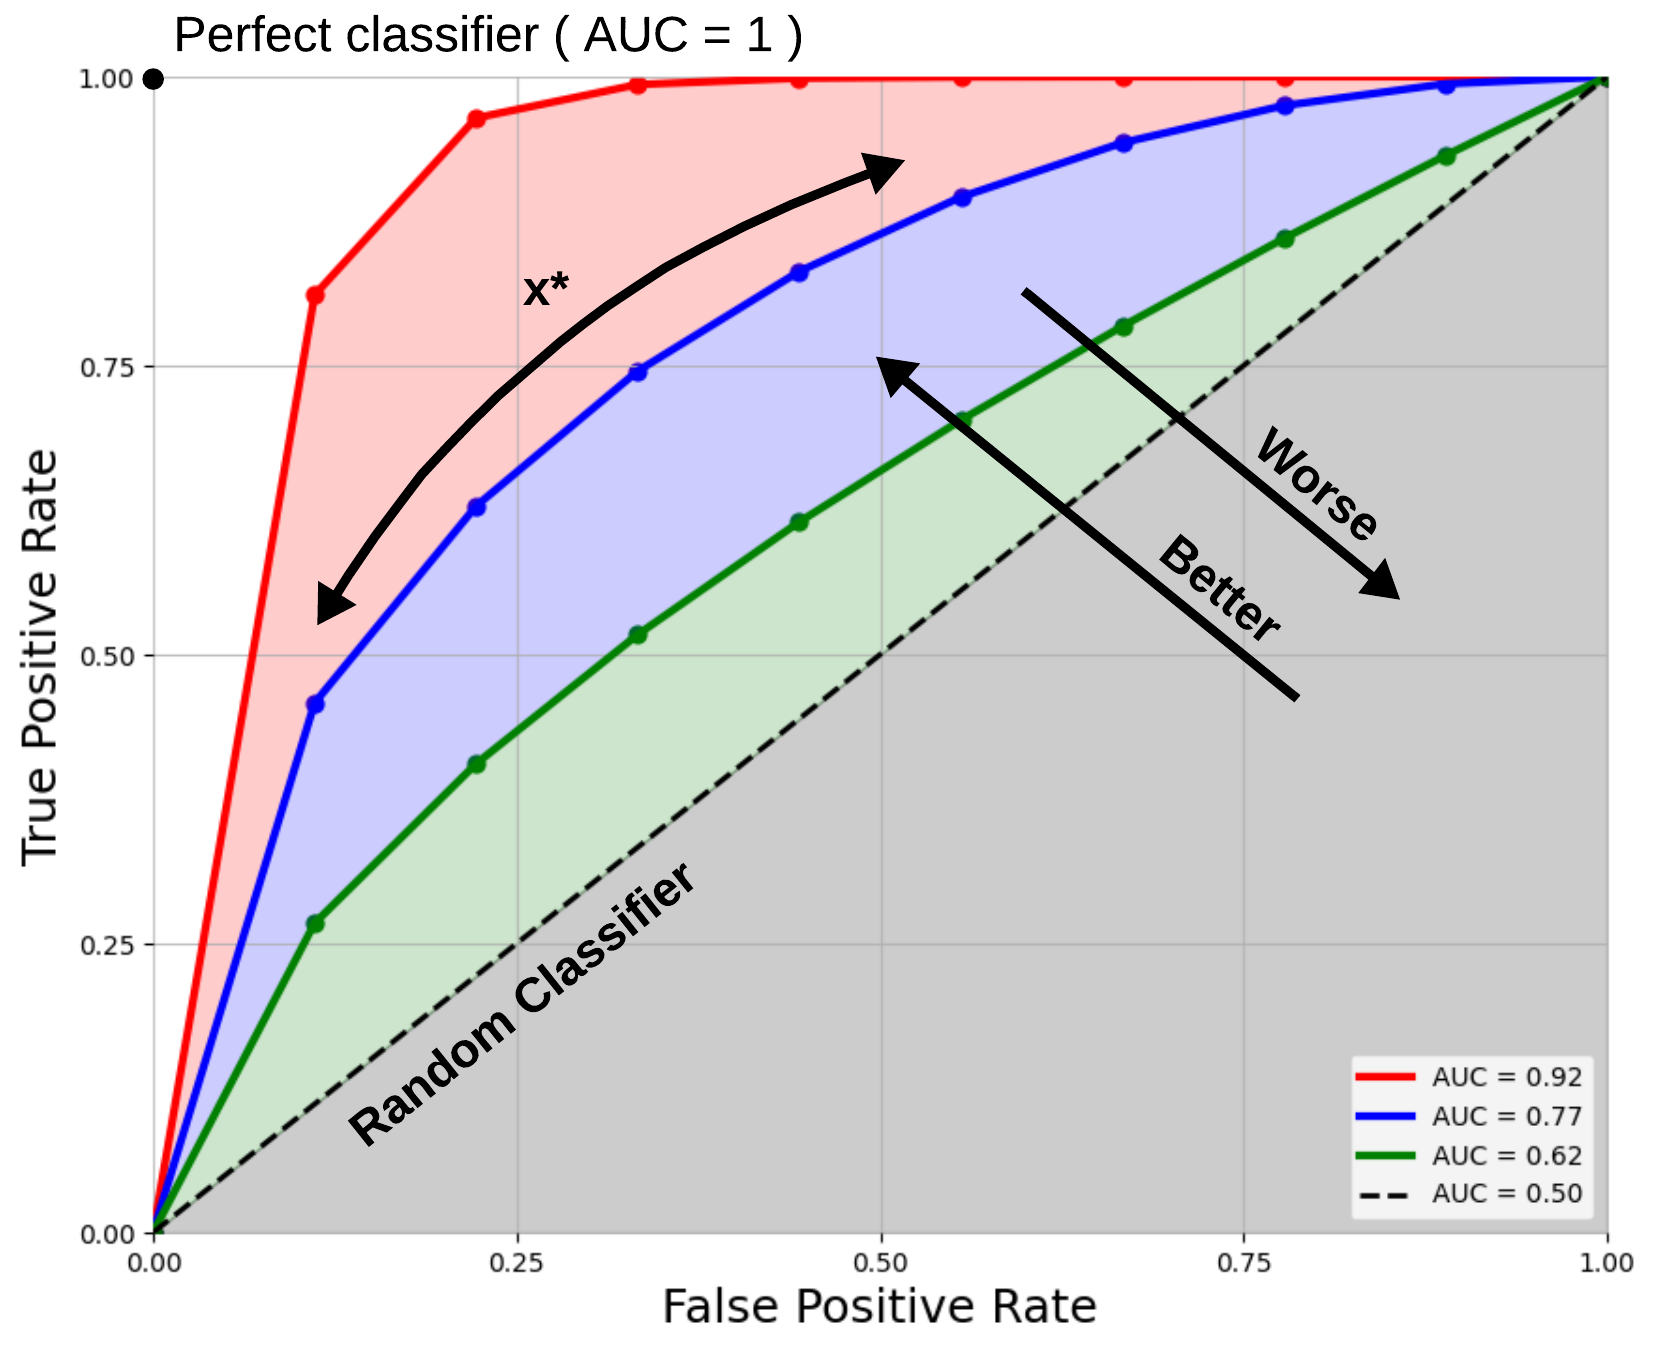
\includegraphics[width=\linewidth]{graphics/ROC_AUC.png}
    \caption{}
    \label{fig:ROC_AUC}
  \end{subfigure}
  \begin{subfigure}{0.65\linewidth}
    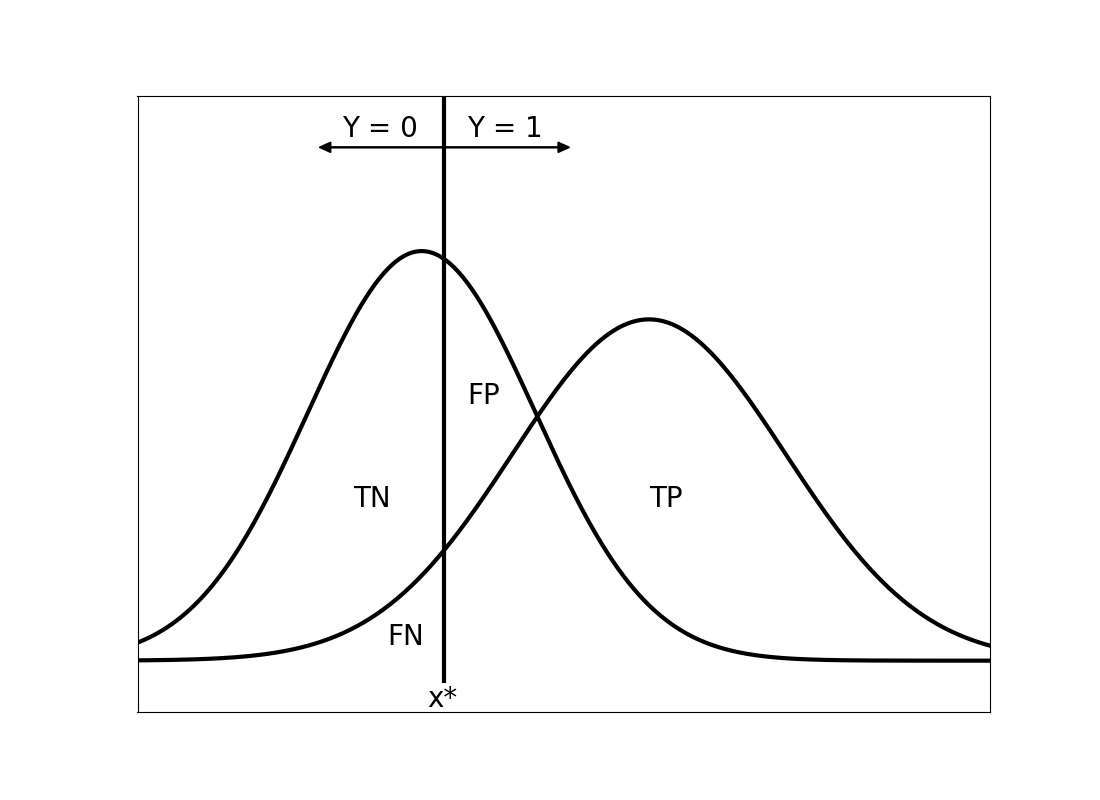
\includegraphics[width=\linewidth]{graphics/PN_Distribution_Thresholded.png}
    \caption{}
    \label{fig:PNDistribution}
  \end{subfigure}
  \caption{ROC curves, AUC and thresholds applied on the data distribution}
  \label{fig:ROC}
\end{figure}